\documentclass[11pt, a4paper]{article}
\usepackage[margin=1in]{geometry}
\usepackage{amsmath, amssymb, amsthm}
\usepackage{tikz}
\usetikzlibrary{calc, intersections, angles, quotes}
\usepackage{enumitem}
\usepackage{fancyhdr}

\pagestyle{fancy}
\fancyhf{}
\rhead{KTOM Juli 2015}
\lhead{Penulis: Idham Muqoddas}
\cfoot{\thepage}

\title{\textbf{Soal dan Pembahasan KTOM Juli 2015}}
\author{\textbf{Penulis:} Idham Muqoddas \\ \textbf{Sumber Soal:} KTOM (ktom-tomi.or.id)}
\date{}

\begin{document}

\maketitle

\section*{Bagian A: Isian}

\begin{enumerate}[label=\textbf{No. \arabic*}, leftmargin=*]
    \item Diberikan segitiga siku-siku $ABC$ di mana $M$ adalah titik tengah sisi miring $AC$. Titik $P, Q, R, S, T, U$ diberikan di luar segitiga ini demikian sehingga $ABPQ, BCRS$, dan $CATU$ merupakan bujur sangkar. Diketahui bahwa hasil jumlah luas ketiga bujur sangkar ini adalah 968. Tentukan panjang $MB$.

    \item Tentukan banyaknya bilangan asli di dalam himpunan $\{1, 2, \dots, 1000\}$ yang hasil jumlah digit-digitnya habis dibagi 3. Sebagai contoh, bilangan 12 jumlah digitnya habis dibagi 3, sementara 20 tidak.

    \item Diberikan segitiga lancip $ABC$ dengan titik pusat lingkaran dalam $I$. Diketahui bahwa $\angle BIC = 110^\circ$. Tentukan besar $\angle BAC$.

    \item Misalkan $r, s, t$ adalah akar-akar dari polinom $p(x) = x^3 - x - 127$. Tentukan nilai dari
    \[ \left(r + \frac{1}{s}\right) \left(s + \frac{1}{t}\right) \left(t + \frac{1}{r}\right). \]

    \item Di Banjarmasin, nomor plat kendaraan diawali dengan huruf DA, diikuti dengan sebuah bilangan 4 digit yang tidak diawali dengan angka 0, dan diakhiri dengan 2 huruf dengan syarat:
    (i) bilangan dari 4 digit tersebut tidak habis dibagi 5 dan
    (ii) dua huruf terakhir tidak boleh konsonan keduanya.
    Misalkan banyaknya kemungkinan nomor plat kendaraan adalah $N$. Tentukan $\lceil \frac{N}{1000} \rceil$.

    \item Misalkan $ABCD$ merupakan sebuah persegi dengan titik pusat $O$. Titik $P$ diberikan di dalam persegi $ABCD$ sehingga $\angle OPB = 45^\circ$. Diketahui $PO = 40\sqrt{2}$ dan $PA = 20$. Tentukan panjang $PB$.

    \item Suatu segitiga memiliki panjang sisi berupa bilangan bulat positif. Diketahui bahwa 5 dan 10 merupakan panjang salah dua dari sisinya dan $s$ merupakan panjang sisi yang satu lagi. Tentukan hasil jumlah semua nilai $s$ yang mungkin.

    \item Terdapat 17 kota yang dapat dituju dari kota Jakarta dengan Olim Air. Diketahui bahwa jika terdapat $k$ orang yang akan berangkat dari kota Jakarta ke 17 kota tujuan ini, pasti ada dua kota tujuan yang banyak penumpangnya sama (bisa jadi tidak terdapat penumpang sama sekali; dalam hal ini banyaknya penumpang adalah 0). Tentukan nilai terbesar $k$ yang mungkin.

    \item Diberikan persegi $ABCD$. Garis singgung dari titik $C$ terhadap lingkaran luar segitiga $ACD$ bertemu dengan perpanjangan garis $AB$ di $E$, dan titik $F$ adalah titik pertemuan kedua lingkaran luar segitiga $BCD$ dengan garis $DE$. Tentukan nilai $EF \times DF$, jika diketahui $|EC| = 21$.

    \item Misalkan $x$ merupakan bilangan real sehingga $2^x + 4^x + 8^x = 1$. Tentukan nilai dari $2^{x+1} - 2^{4x}$.

    \item Bilangan asli $k$ disebut keras jika memenuhi sifat bahwa: tidak terdapat bilangan asli $a, b$ sehingga $a + b + ab = k$. Tentukan banyaknya bilangan keras di dalam himpunan $\{1, 2, 3, \dots, 100\}$.

    \item Di toko buah Piade Mart, Anda ingin membeli 35 buah. Toko buah tersebut menjual 5 macam buah: pepaya, nanas, semangka, apel, melon. Ada aturan-aturan ketika melakukan pembelian.
    1. pepaya yang dibeli harus sebanyak kelipatan 5,
    2. nanas yang dibeli maksimal 4,
    3. semangka yang dibeli harus berjumlah genap,
    4. apel yang dibeli maksimal 1.
    Berapa banyak cara membeli buah-buahan jika semua aturan di atas terpenuhi?

    \item Diberikan titik $P(-2, r)$ dan $R(4, 4)$ pada bidang-xy dengan $r$ suatu bilangan real positif. Jika titik $Q$ terletak pada sumbu-x, maka nilai terkecil yang mungkin untuk $|PQ| + |QR|$ adalah 10. Tentukan hasil jumlah semua nilai $r$ yang mungkin.

    \item Pada sebuah segitiga $ABC$, titik $D, E$ dipilih pada segmen garis $BC$ sehingga $AD = AE$ dengan titik $D, E$ dalam urutan $B, D, E, C$. Diketahui $AB = 43$, $AC = 27$, dan $BD - CE = 20$. Tentukan panjang $BC$.

    \item Sebuah turnamen tenis diikuti 6 pemain sehingga setiap pemain berhadapan satu sama lain tepat sekali. Untuk setiap permainan, pasti salah satu pemain menang dan yang satu lagi kalah. Misalkan $N$ adalah banyaknya kemungkinan hasil semua pertandingan sehingga tidak ada pemain yang tidak terkalahkan. Tentukan tiga digit terakhir dari $N$.

    \item Ada 21 petak yang berurutan dari kiri ke kanan, bernomor $0, 1, \dots, 20$. Seekor kelinci, mulai dari petak ke-0, ingin mencapai petak ke-20, dimana ia hanya dapat melompat 1 atau 2 petak ke depan saja. Misalkan $n$ banyaknya cara kelinci tersebut mencapai petak ke-20, tanpa menginjak petak ke-15. Hitung sisa $n$ ketika dibagi 1000.

    \item Diberikan sebuah kertas berukuran persegi panjang. Jika kertas tersebut dilipat terhadap diagonalnya, akan terbentuk suatu segilima yang luasnya $\frac{11}{16}$ dari luas persegi panjang awal. Jika lebar dari persegi panjang tersebut adalah 13, tentukan luas persegi panjang tersebut.

    \item Diberikan suatu himpunan $S = \{1, 11, 111, 1111, \dots\}$, yaitu himpunan semua bilangan asli yang digit-digitnya adalah 1. Suatu bilangan disebut bersifat \textit{kuat} jika bilangan tersebut membagi habis setidaknya satu dari anggota himpunan $S$. Ada berapakah bilangan kuat yang merupakan anggota himpunan $\{1, 2, \dots, 1000\}$?

    \item Diketahui suatu bilangan real $a, b, c,$ dan $d$ memenuhi
    \[ \frac{a - b}{c - d} = 2 \quad \text{dan} \quad \frac{a - c}{b - d} = 3. \]
    Tentukan hasil jumlah semua nilai yang mungkin untuk $\frac{a - d}{b - c}$.

    \item Diberikan segitiga $ABC$ dengan $BC = 20$ dan misalkan $D$ merupakan titik tengah $BC$. Lingkaran dalam segitiga $ABC$ memotong segmen garis $AD$ menjadi tiga potong yang sama panjang. Misalkan $a$ merupakan luas dari segitiga $ABC$. Tentukan tiga digit terakhir dari $a^2$.

    \item Tentukan hasil penjumlahan dari semua bilangan asli $n$ yang memenuhi $n - \varphi(n) = 15$. Notasi $\varphi(n)$ menyatakan banyaknya bilangan asli yang kurang dari $n$ dan relatif prima dengan $n$. Sebagai contoh, $\varphi(12) = 4$.
\end{enumerate}

\section*{Bagian B: Esai}

\begin{enumerate}[label=\textbf{No. \arabic*}, leftmargin=*]
    \item Untuk setiap bilangan asli $n$, misalkan $d(n)$ menyatakan banyaknya bilangan asli yang habis membagi $n$. Sebagai contoh, jika $n = 6$, maka $d(n) = 4$. Jika $n$ memiliki bentuk aritmetika $p_1^{a_1} p_2^{a_2} \dots p_k^{a_k}$ dengan $p_1, p_2, \dots, p_k$ merupakan bilangan prima berbeda dan $a_1, a_2, \dots, a_k$ merupakan bilangan asli, dapat ditunjukkan bahwa $d(n) = (a_1 + 1)(a_2 + 1) \dots (a_k + 1)$.
    \begin{enumerate}[label=\arabic*.]
        \item Tentukan nilai dari $d(2015^{2015})$.
        \item Misalkan $m$ merupakan bilangan asli sehingga $d(m) = 2015^{2015}$. Berikan satu buah contoh $m$ yang memenuhi.
        \item Misalkan $m$ merupakan bilangan asli sehingga $d(m) = 2015^{2015}$. Haruskah $m$ merupakan bilangan kuadrat sempurna?
    \end{enumerate}

    \item Di sebuah turnamen sepakbola, setiap tim bertanding melawan tim lainnya tepat sekali, kemenangan diganjar 3 poin, seri diganjar 1 poin, dan kekalahan tidak diganjar poin. Diketahui di akhir turnamen, Euclid United menjadi juara 1 dengan 8 poin, Trigonspor menjadi juara 2 dengan 7 poin, Analit FC menjadi juara 3 dengan 4 poin, dan Real Kompleks menempati peringkat 4 dengan 4 poin. Tentukan semua kemungkinan banyak tim sepakbola di turnamen ini.

    \item Misalkan $x$ dan $y$ merupakan bilangan real dengan $xy \neq -1$ demikian sehingga
    \[ \frac{x^5y + xy^5}{1 + x^3y^3} = 2. \]
    Tentukan nilai terkecil yang mungkin untuk $x^2 + y^2$.
\end{enumerate}

\newpage
\section*{Pembahasan}

\subsection*{Bagian A: Isian}

\textbf{No. 1}\\
Misalkan sisi $\triangle ABC$ adalah $AB = c$, $BC = a$, dan $AC = b$. Karena siku-siku di $B$, berlaku $a^2 + c^2 = b^2$.
Luas ketiga bujur sangkar adalah $AB^2 + BC^2 + AC^2 = c^2 + a^2 + b^2 = 2b^2$.
Diketahui jumlah luas tersebut 968, sehingga $2b^2 = 968 \implies b^2 = 484 \implies b = 22$.
Pada segitiga siku-siku, panjang garis berat yang ditarik dari sudut siku-siku ke sisi miring sama dengan setengah dari sisi miringnya. Sehingga $MB = \frac{AC}{2} = \frac{22}{2} = 11$.

\begin{center}
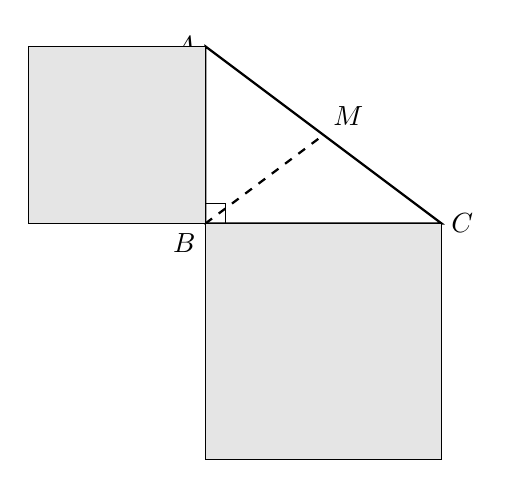
\begin{tikzpicture}[scale=0.25]
\coordinate (B) at (0,0);
\coordinate (C) at (12,0);
\coordinate (A) at (0,9);
\coordinate (M) at (6,4.5);
\draw[thick] (A) -- (B) -- (C) -- cycle;
\draw[thick, dashed] (B) -- (M);
\node[left] at (A) {$A$};
\node[below left] at (B) {$B$};
\node[right] at (C) {$C$};
\node[above right] at (M) {$M$};
\draw (0,1) -- (1,1) -- (1,0);
\draw[fill=gray!20] (A) -- (-9,9) -- (-9,0) -- (B) -- cycle;
\draw[fill=gray!20] (B) -- (0,-12) -- (12,-12) -- (C) -- cycle;
\coordinate (A') at ($(A) + (C) - (B) + (9, 12)$); % Just approximation for illustrative bounding box
\end{tikzpicture}
\end{center}

\textbf{No. 2}\\
Sifat bilangan yang jumlah digit-digitnya habis dibagi 3 adalah bilangan tersebut sendiri habis dibagi 3.
Banyaknya bilangan kelipatan 3 pada himpunan $\{1, 2, \dots, 1000\}$ adalah $\lfloor \frac{1000}{3} \rfloor = 333$.

\textbf{No. 3}\\
Titik $I$ adalah pusat lingkaran dalam (incenter), yang merupakan titik potong garis bagi sudut. Pada $\triangle ABC$, sudut $\angle BIC$ memenuhi hubungan $\angle BIC = 90^\circ + \frac{\angle BAC}{2}$.
Substitusi nilai yang diketahui: $110^\circ = 90^\circ + \frac{\angle BAC}{2} \implies \frac{\angle BAC}{2} = 20^\circ \implies \angle BAC = 40^\circ$.

\begin{center}
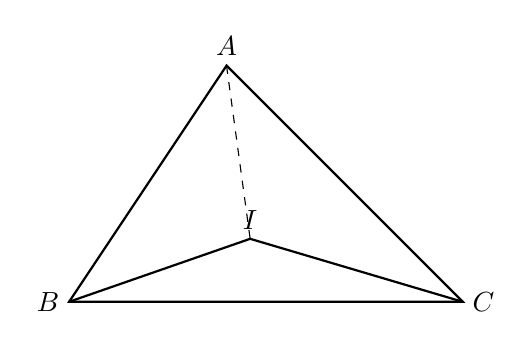
\begin{tikzpicture}[scale=1]
\coordinate (A) at (0,3);
\coordinate (B) at (-2,0);
\coordinate (C) at (3,0);
\draw[thick] (A) -- (B) -- (C) -- cycle;
\coordinate (I) at (0.3,0.8);
\draw[thick] (B) -- (I) -- (C);
\node[above] at (A) {$A$};
\node[left] at (B) {$B$};
\node[right] at (C) {$C$};
\node[above] at (I) {$I$};
\draw[dashed] (A) -- (I);
\end{tikzpicture}
\end{center}

\textbf{No. 4}\\
Kita jabarkan ekspresi yang ditanyakan:
\[ \left(r + \frac{1}{s}\right) \left(s + \frac{1}{t}\right) \left(t + \frac{1}{r}\right) = rst + r + s + t + \frac{1}{r} + \frac{1}{s} + \frac{1}{t} + \frac{1}{rst} \]
Berdasarkan Teorema Vieta pada $p(x) = x^3 - x - 127 = 0$, kita memiliki:
$r+s+t = 0$, $rs+st+tr = -1$, dan $rst = 127$.
Sehingga, $\frac{1}{r} + \frac{1}{s} + \frac{1}{t} = \frac{rs+st+tr}{rst} = \frac{-1}{127}$.
Substitusi ke bentuk awal:
$127 + 0 + \left(-\frac{1}{127}\right) + \frac{1}{127} = 127$.

\textbf{No. 5}\\
- \textbf{Bagian angka}: Terdapat 9000 kemungkinan bilangan 4 digit (dari 1000 hingga 9999). Agar tidak habis dibagi 5, angka terakhir tidak boleh 0 dan 5, sehingga tersisa 8 pilihan angka terakhir. Banyak kemungkinan = $9 \times 10 \times 10 \times 8 = 7200$. \\
- \textbf{Bagian huruf}: Ada 2 huruf, total kemungkinan $26 \times 26 = 676$. Huruf konsonan berjumlah 21. Banyak kemungkinan di mana kedua hurufnya konsonan adalah $21 \times 21 = 441$. Syarat (ii) melarang ini, sehingga kemungkinannya $676 - 441 = 235$.\\
$N = 7200 \times 235 = 1.692.000$. Nilai $\lceil \frac{N}{1000} \rceil = 1692$.

\textbf{No. 6}\\
Misalkan jarak $OB = x$. Dengan Aturan Kosinus pada $\triangle POB$:
$OB^2 = OP^2 + PB^2 - 2 \cdot OP \cdot PB \cos 45^\circ \implies x^2 = 3200 + PB^2 - 80PB$.
Dengan Aturan Kosinus pada $\triangle POA$ (dengan mengingat $\angle POA = 90^\circ - \angle POB$):
$PA^2 = OP^2 + OA^2 - 2 \cdot OP \cdot OA \cos(90^\circ - \angle POB) = OP^2 + x^2 - 2 \cdot OP \cdot x \sin \angle POB$.
Berdasarkan kesamaan luas, $\frac{1}{2} OP \cdot x \sin \angle POB = \text{Luas }\triangle POB = \frac{1}{2} OP \cdot PB \sin 45^\circ \implies x \sin \angle POB = \frac{PB}{\sqrt{2}}$.
Sehingga: $PA^2 = 3200 + x^2 - 2(40\sqrt{2})\left(\frac{PB}{\sqrt{2}}\right) \implies 400 = 3200 + x^2 - 80PB$.
Substitusi $x^2 = 3200 + PB^2 - 80PB$:
$400 = 3200 + (3200 + PB^2 - 80PB) - 80PB \implies PB^2 - 160PB + 6000 = 0$.
Akar-akarnya $PB = 60$ atau $PB = 100$. Karena titik $P$ harus berada di dalam persegi, hanya $PB = 100$ yang secara geometris memenuhi sehingga titik tidak terlempar ke luar persegi (jarak pusat ke sudut). Jadi $PB = 100$.

\begin{center}
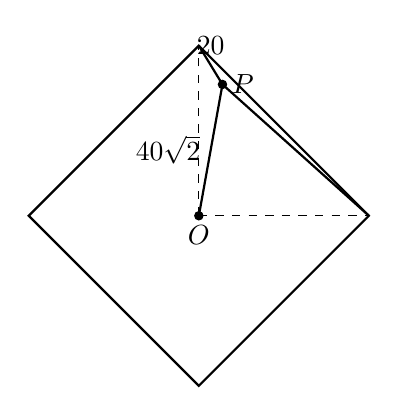
\begin{tikzpicture}[scale=0.03]
\coordinate (O) at (0,0);
\coordinate (B) at (72,0);
\coordinate (A) at (0,72);
\coordinate (C) at (0,-72);
\coordinate (D) at (-72,0);
\draw[thick] (A) -- (B) -- (C) -- (D) -- cycle;
\coordinate (P) at (10, 55.6); % approximate
\draw[fill] (O) circle (50pt) node[below] {$O$};
\draw[fill] (P) circle (50pt) node[right] {$P$};
\draw[thick] (O) -- (P) node[midway, left] {$40\sqrt{2}$};
\draw[thick] (P) -- (B);
\draw[thick] (P) -- (A) node[midway, above] {$20$};
\draw[dashed] (O) -- (B);
\draw[dashed] (O) -- (A);
\end{tikzpicture}
\end{center}

\textbf{No. 7}\\
Berdasarkan ketaksamaan segitiga, nilai $s$ memenuhi $|10 - 5| < s < 10 + 5 \implies 5 < s < 15$.
Karena $s$ bilangan bulat, maka $s \in \{6, 7, 8, 9, 10, 11, 12, 13, 14\}$.
Jumlahnya $= 6 + 7 + 8 + 9 + 10 + 11 + 12 + 13 + 14 = 90$.

\textbf{No. 8}\\
Agar pasti ada dua kota dengan penumpang sama berapapun distribusinya, total penumpang $k$ tidak boleh bisa dipecah menjadi 17 bilangan bulat non-negatif berbeda. Penjumlahan 17 bilangan bulat non-negatif berbeda yang terkecil adalah $0 + 1 + 2 + \dots + 16 = 136$.
Maka, jika $k < 136$, mustahil ke-17 kota memiliki penumpang berbeda. Nilai terbesar $k$ adalah 135.

\textbf{No. 9}\\
Perhatikan bahwa lingkaran luar $\triangle ACD$ dan lingkaran luar $\triangle BCD$ adalah lingkaran yang sama, yakni lingkaran luar persegi $ABCD$. Misalkan sisi persegi adalah $s$. Garis singgung di $C$ memotong perpanjangan $AB$ di $E$, sehingga $\triangle BCE$ siku-siku dan sebangun. Sifat garis singgung pada titik sudut memotong perpanjangan sumbu mendatar sedemikian hingga jarak $B$ ke $E$ adalah $s$. Maka $EC = s\sqrt{2}$. Karena $|EC| = 21$, maka $s^2 = \frac{441}{2}$.
Titik $D, C, F$ berada pada lingkaran. Teorema Kuasa Titik untuk $E$ di luar lingkaran memberikan $ED \times EF = EC^2 = 441$.
Pada segitiga siku-siku $\triangle ADE$, $AD = s$ dan $AE = 2s$, sehingga $ED = s\sqrt{5}$.
Kita tahu $EF = \frac{EC^2}{ED}$. Panjang $DF = ED - EF$.
$EF \times DF = \frac{EC^2}{ED} \left( ED - \frac{EC^2}{ED} \right) = EC^2 - \frac{EC^4}{ED^2} = 441 - \frac{441^2}{5s^2} = 441 - \frac{441^2}{5(441/2)} = 441 - \frac{2 \cdot 441}{5} = \frac{3 \times 441}{5} = \frac{1323}{5} = 264.6$.

\begin{center}
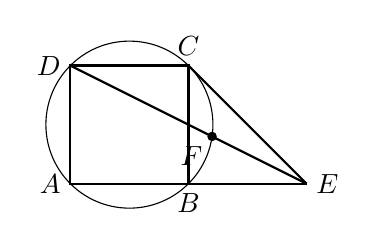
\begin{tikzpicture}[scale=0.15]
\coordinate (A) at (0,0);
\coordinate (B) at (10,0);
\coordinate (C) at (10,10);
\coordinate (D) at (0,10);
\coordinate (E) at (20,0);
\coordinate (O) at (5,5);
\draw[thick] (A) -- (B) -- (C) -- (D) -- cycle;
\draw[thick] (B) -- (E);
\draw (O) circle (7.071);
\draw[thick] (C) -- (E);
\draw[thick] (D) -- (E);
\coordinate (F) at (12, 4); % approx
\draw[fill] (F) circle (10pt) node[below left] {$F$};
\node[left] at (A) {$A$};
\node[below] at (B) {$B$};
\node[above] at (C) {$C$};
\node[left] at (D) {$D$};
\node[right] at (E) {$E$};
\end{tikzpicture}
\end{center}

\textbf{No. 10}\\
Misalkan $y = 2^x$. Persamaan menjadi $y + y^2 + y^3 = 1$.
Kalikan dengan $(y-1)$ memberikan: $(y-1)(y^3+y^2+y) = y-1 \implies y^4 - y = y - 1 \implies y^4 = 2y - 1$.
Maka nilai $2^{x+1} - 2^{4x} = 2y - y^4 = 2y - (2y - 1) = 1$.

\textbf{No. 11}\\
Persamaan $a+b+ab = k$ ekuivalen dengan $(a+1)(b+1) = k+1$.
Bilangan $k$ "keras" jika $k+1$ tidak bisa difaktorkan menjadi perkalian dua bilangan $\ge 2$, dengan kata lain $k+1$ adalah bilangan prima.
Karena $k \in \{1, 2, \dots, 100\}$, kita mencari banyak bilangan prima di selang $2 \le p \le 101$.
Banyaknya bilangan prima $\le 100$ adalah 25. Angka 101 juga prima. Maka total ada 26 bilangan keras.

\textbf{No. 12}\\
Ini adalah permasalahan fungsi pembangkit (Generating Function). Syarat koefisien:
Pepaya (P): $1 + x^5 + x^{10} + \dots = \frac{1}{1-x^5}$ \\
Nanas (N): $1 + x + x^2 + x^3 + x^4 = \frac{1-x^5}{1-x}$ \\
Semangka (S): $1 + x^2 + x^4 + \dots = \frac{1}{1-x^2}$ \\
Apel (A): $1 + x$ \\
Melon (M): $1 + x + x^2 + \dots = \frac{1}{1-x}$ \\
Kalikan kelimanya: $\frac{1}{1-x^5} \cdot \frac{1-x^5}{1-x} \cdot \frac{1}{1-x^2} \cdot (1+x) \cdot \frac{1}{1-x} = \frac{1+x}{(1-x)^3 (1-x^2)} = \frac{1}{(1-x)^4}$.
Kita mencari koefisien $x^{35}$ pada penjabaran $(1-x)^{-4}$.
Nilainya adalah $\binom{35+4-1}{4-1} = \binom{38}{3} = \frac{38 \times 37 \times 36}{3 \times 2 \times 1} = 8436$.

\textbf{No. 13}\\
Jarak terpendek $|PQ| + |QR|$ diperoleh ketika memantulkan $P$ terhadap sumbu-x menjadi $P'(-2, -r)$.
Jarak lurus $P'R = \sqrt{(4 - (-2))^2 + (4 - (-r))^2} = \sqrt{36 + (4+r)^2}$.
Karena minimum tersebut adalah 10, maka $36 + (r+4)^2 = 100 \implies (r+4)^2 = 64$.
Akar-akarnya $r+4 = 8 \implies r=4$ atau $r+4 = -8 \implies r = -12$.
Karena $r$ bilangan real positif, maka $r = 4$. Jumlah semua nilai $r$ yang mungkin adalah 4.

\begin{center}
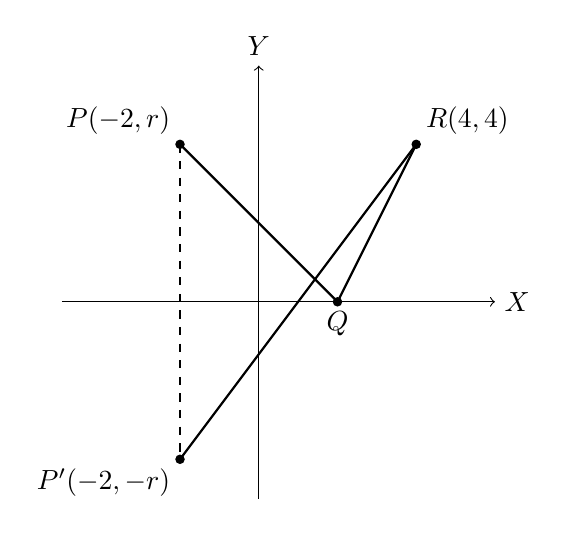
\begin{tikzpicture}[scale=0.5]
\draw[->] (-5,0) -- (6,0) node[right] {$X$};
\draw[->] (0,-5) -- (0,6) node[above] {$Y$};
\coordinate (P) at (-2,4);
\coordinate (R) at (4,4);
\coordinate (P') at (-2,-4);
\draw[fill] (P) circle (3pt) node[above left] {$P(-2,r)$};
\draw[fill] (R) circle (3pt) node[above right] {$R(4,4)$};
\draw[fill] (P') circle (3pt) node[below left] {$P'(-2,-r)$};
\draw[dashed] (P) -- (P');
\draw[thick] (P') -- (R);
\draw[thick] (P) -- (2,0) -- (R);
\node[below] at (2,0) {$Q$};
\draw[fill] (2,0) circle (3pt);
\end{tikzpicture}
\end{center}

\textbf{No. 14}\\
Tarik garis tinggi $AM$ tegak lurus $BC$. Karena $\triangle ADE$ sama kaki ($AD=AE$), maka $M$ adalah titik tengah $DE$, yang berarti $DM = EM$.
Teorema Pythagoras pada $\triangle ABM$ dan $\triangle ACM$:
$AM^2 = AB^2 - BM^2 = AC^2 - CM^2 \implies BM^2 - CM^2 = 43^2 - 27^2 = 1120$.
Perhatikan bahwa $BM = BD + DM$ dan $CM = CE + EM$. Karena $DM = EM$, $BM - CM = BD - CE = 20$.
Maka $BM^2 - CM^2 = (BM - CM)(BM + CM) = 20(BM + CM) = 1120 \implies BM + CM = 56$.
Panjang $BC = BM + CM = 56$.

\begin{center}
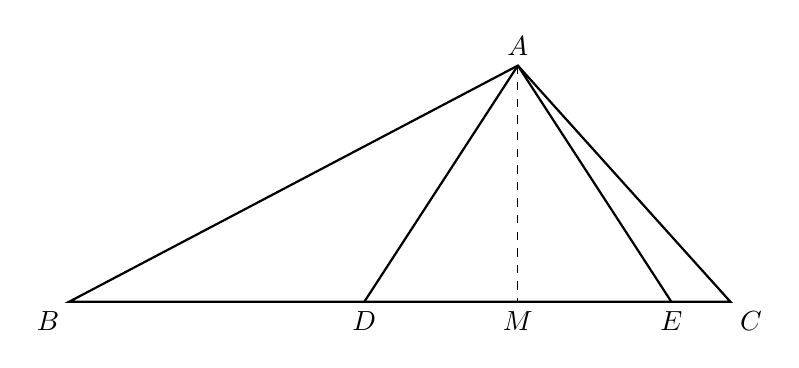
\begin{tikzpicture}[scale=0.15]
\coordinate (B) at (0,0);
\coordinate (C) at (56,0);
\coordinate (M) at (38,0);
\coordinate (A) at (38, 20); % approx
\draw[thick] (A) -- (B) -- (C) -- cycle;
\coordinate (D) at (25,0);
\coordinate (E) at (51,0);
\draw[thick] (A) -- (D);
\draw[thick] (A) -- (E);
\draw[dashed] (A) -- (M);
\node[above] at (A) {$A$};
\node[below left] at (B) {$B$};
\node[below] at (D) {$D$};
\node[below] at (M) {$M$};
\node[below] at (E) {$E$};
\node[below right] at (C) {$C$};
\end{tikzpicture}
\end{center}

\textbf{No. 15}\\
Total pertandingan adalah $\binom{6}{2} = 15$, sehingga total hasil adalah $2^{15} = 32768$.
"Pemain yang tidak terkalahkan" berarti ia menang 5 kali. Hanya mungkin maksimal ada 1 orang seperti itu.
Banyak cara memilih 1 orang yang menang terus adalah 6. Sisa 5 orang lainnya memiliki $\binom{5}{2} = 10$ pertandingan antar mereka, menghasilkan $2^{10} = 1024$ hasil.
Banyak kemungkinan ada pemenang mutlak adalah $6 \times 1024 = 6144$.
$N = 32768 - 6144 = 26624$. Tiga digit terakhirnya adalah 624.

\textbf{No. 16}\\
Masalah ini ekuivalen dengan barisan Fibonacci $F_n$. Cara mencapai petak $n$ tanpa larangan adalah $F_n$ (dengan $F_0 = F_1 = 1, F_2 = 2$).
Agar tidak menginjak petak ke-15, kelinci harus mendarat di petak ke-14, lalu dipaksa melompat 2 langkah ke petak ke-16, lalu lanjut ke petak ke-20.
Banyak cara adalah $F_{14} \times 1 \times F_4$.
Dengan menghitung deret, $F_4 = 5$ dan $F_{14} = 610$.
$n = 610 \times 5 = 3050$. Sisa ketika dibagi 1000 adalah 050.

\textbf{No. 17}\\
Misalkan persegi panjang $ABCD$ berukuran $l \times w$ dengan $w = 13$. Saat dilipat menurut $AC$, terbentuk daerah tumpang tindih berupa segitiga sama kaki $\triangle AEC$ dengan area $T$.
Luas segilima yang terbentuk adalah $Luas(ABCD) - T$.
Didapat $lw - T = \frac{11}{16} lw \implies T = \frac{5}{16} lw$.
Pada $\triangle AEC$, $AE = EC = x$. Menggunakan Pythagoras pada $\triangle EBC$: $(l-x)^2 + w^2 = x^2 \implies x = \frac{l^2+w^2}{2l}$.
$T = \frac{1}{2} w \cdot x = \frac{w(l^2+w^2)}{4l}$.
$\frac{w(l^2+w^2)}{4l} = \frac{5}{16} lw \implies \frac{l^2+w^2}{l} = \frac{5}{4} l \implies l = 2w$.
Karena $w = 13$, maka $l = 26$. Luas awal $= 26 \times 13 = 338$.

\textbf{No. 18}\\
Suatu bilangan membagi setidaknya salah satu $(10^k-1)/9$ jika dan hanya jika ia relatif prima dengan 10 (tidak habis dibagi 2 dan 5) berdasar Teorema Euler. Bilangan kuat hanyalah bilangan yang $\gcd(n, 10) = 1$.
Pada rentang $\{1, 2, \dots, 1000\}$, banyaknya adalah $1000 \times \frac{\varphi(10)}{10} = 1000 \times \frac{4}{10} = 400$.

\textbf{No. 19}\\
Diberikan: $a-b = 2(c-d)$ dan $a-c = 3(b-d)$.
Kurangkan persamaan pertama dan kedua: $c - b = 2c - 3b + d \implies d = 2b - c$.
Substitusi $d$ ke persamaan pertama: $a - b = 2c - 2(2b - c) \implies a = 4c - 3b$.
Yang dicari: $\frac{a-d}{b-c} = \frac{(4c-3b) - (2b-c)}{b-c} = \frac{5c-5b}{b-c} = -5$.

\textbf{No. 20}\\
Misalkan lingkaran dalam menyinggung $BC$ di $T$. Panjang garis singgung dari $D$ (karena $D$ berada pada sisi bersinggungan di luar lingkaran dalam) adalah $DT$. Karena lingkaran memotong $AD$ menjadi 3 segmen $x$ yang sama ($AD = 3x$), kuasa titik dari $D$ bernilai $x \cdot 2x = 2x^2$, begitu pula kuasa titik dari $A$ bernilai $2x^2$. Oleh karena itu garis singgung dari $A$ ke lingkaran dalam (yakni $s-a$) harus sama panjang dengan $DT$.
Diketahui $DT = |BD - BT| = \left|10 - \frac{a+c-b}{2}\right| = \frac{|b-c|}{2}$.
Dari sini $(s-a)^2 = DT^2 \implies \frac{b+c-20}{2} = \frac{b-c}{2} \implies c = 10$ (asumsikan $b>c$).
Teorema Apollonius memberikan $AD^2 = \frac{2b^2 + 2c^2 - a^2}{4} = \frac{b^2 - 100}{2}$.
Karena $(s-a)^2 = \frac{2}{9} AD^2$, $\frac{(b-10)^2}{4} = \frac{b^2-100}{9} \implies 9(b-10) = 4(b+10) \implies b = 26$.
Luas segitiga dengan Heron $s = 28$: $a^2 = 28(8)(2)(18) = 8064$.
Tiga digit terakhir: 064.

\begin{center}
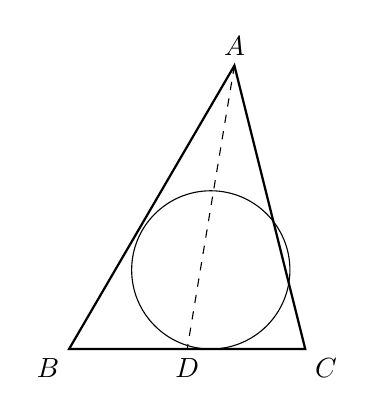
\begin{tikzpicture}[scale=0.15]
\coordinate (B) at (0,0);
\coordinate (C) at (20,0);
\coordinate (D) at (10,0);
\coordinate (A) at (14, 24); % approx
\draw[thick] (A) -- (B) -- (C) -- cycle;
\draw[dashed] (A) -- (D);
\draw (12, 6.7) circle (6.7); % Incircle approximation
\node[above] at (A) {$A$};
\node[below left] at (B) {$B$};
\node[below right] at (C) {$C$};
\node[below] at (D) {$D$};
\end{tikzpicture}
\end{center}

\textbf{No. 21}\\
Kita memecah kasus untuk $n-\varphi(n) = 15$. Jika $n$ genap, maka $\varphi(n)$ juga genap, sehingga selisihnya genap (kontradiksi). Maka $n$ pasti ganjil.
Jika $n = pq$, $n - (p-1)(q-1) = p + q - 1 = 15 \implies p + q = 16$.
Kombinasi prima ganjil $(p,q)$ yang berjumlah 16 adalah (3, 13) dan (5, 11).
Menghasilkan $n = 39$ dan $n = 55$. Tidak ada kombinasi prima berpangkat atau $>2$ prima yang memenuhi (karena akan melampaui rentang). Total = $39 + 55 = 94$.


\subsection*{Bagian B: Esai}

\textbf{No. 1}
\begin{enumerate}[label=\arabic*.]
    \item Faktorisasi prima $2015 = 5 \times 13 \times 31$.
    Maka $2015^{2015} = 5^{2015} 13^{2015} 31^{2015}$.
    Banyaknya faktor positif adalah $d = (2015+1)(2015+1)(2015+1) = 2016^3 = 8.193.540.096$.
    \item Contoh $m$: Kita mencari $m$ agar perkalian eksponen ditambah 1 menjadi $2015^{2015}$.
    Karena $2015^{2015} = \underbrace{2015 \times 2015 \times \dots \times 2015}_{2015 \text{ kali}}$, maka kita bisa membuat bilangan dengan 2015 faktor prima berbeda, misalnya $p_1, p_2, \dots, p_{2015}$.
    Salah satu contoh $m = p_1^{2014} \cdot p_2^{2014} \dots p_{2015}^{2014}$, dengan $p_i$ merupakan bilangan prima ke-$i$.
    \item Nilai $2015^{2015}$ adalah bilangan ganjil. Sebuah bilangan genap pembagi (jumlah divisor) bernilai ganjil jika dan hanya jika semua unsur $(a_k + 1)$ pada faktorisasinya adalah ganjil.
    Ini berarti seluruh eksponen $a_k$ merupakan bilangan genap. Bilangan dengan eksponen prima semuanya genap adalah definisi dari bilangan kuadrat sempurna. \textbf{Ya}, $m$ harus merupakan bilangan kuadrat sempurna.
\end{enumerate}

\textbf{No. 2}\\
Misalkan banyak tim adalah $n$. Total pertandingan yang dilakukan adalah $\frac{n(n-1)}{2}$.
Setiap pertandingan memberikan total 3 poin (jika ada yang menang) atau 2 poin (jika seri).
Maka, total poin seluruh tim $P$ berada dalam batas: $n(n-1) \le P \le \frac{3n(n-1)}{2}$.
Poin 4 tim teratas dijumlahkan adalah $8 + 7 + 4 + 4 = 23$. Sehingga $P \ge 23$.
- Jika $n=4$, total poin maksimal $\frac{3(4)(3)}{2} = 18 < 23$ (Mustahil).
- Jika $n=5$, rentang $P$ adalah $20 \le P \le 30$. Tim kelima harus memiliki poin $\le 4$. $P_{total} = 23 + x$. Ini mungkin.
- Jika $n \ge 6$, batas poin minimal poin $P \ge 30$, namun tim ke-5 dan ke-6 maksimal memiliki nilai 4, sehingga $P = 23 + 4 + 4 = 31$. Karena pertandingan banyak yang seri poin maksimal dari satu tim sangat kecil, tidak akan ada yang bisa menembus 8 poin pada kondisi hampir semua seri, menyebabkan kontradiksi struktural grafik turnamen.
Maka, satu-satunya nilai $n$ yang mungkin adalah \textbf{5}.

\textbf{No. 3}\\
Misalkan $p = xy$ dan $s = x^2 + y^2$. Ekspresi numerator dapat ditulis sebagai:
$x^5y + xy^5 = xy(x^4 + y^4) = p((x^2+y^2)^2 - 2x^2y^2) = p(s^2 - 2p^2)$.
Persamaan yang diberikan menjadi: $\frac{p(s^2 - 2p^2)}{1 + p^3} = 2 \implies ps^2 - 2p^3 = 2 + 2p^3 \implies s^2 = 4p^2 + \frac{2}{p}$.
Untuk mencari nilai terkecil $s = x^2+y^2$, kita cari minimum dari $s^2$ menggunakan ketaksamaan AM-GM pada $p > 0$:
$s^2 = 4p^2 + \frac{1}{p} + \frac{1}{p} \ge 3 \sqrt[3]{4p^2 \cdot \frac{1}{p} \cdot \frac{1}{p}} = 3 \sqrt[3]{4}$.
Maka nilai minimum untuk $s^2$ adalah $3 \cdot 2^{2/3}$.
Nilai terkecil dari $x^2 + y^2$ adalah $\sqrt{3 \cdot 2^{2/3}} = \sqrt{3} \cdot \sqrt[3]{2} = \sqrt[6]{108}$.

\end{document}
